
\include{common-handout}

\raggedcolumns

\hypersetup{
  pdftitle={Python in Neuronal Simulation},
}

%%% Body
\begin{document}

\begin{multicols}{3}    % 3 columns

% Document title
%\section*{
\begin{center}\Large \textbf{Python in Neuronal Simulation}\end{center}
%}
%\label{python-in-neuronal-simulation}

\begin{center}
\noindent
\includegraphics[width=0.7\columnwidth]{python_action_potential}
%\includegraphics[width=0.5\columnwidth]{openlogo-vsop}

Find the community @ \url{http://neuralensemble.org}


% \hrule
\end{center}
\vspace{0em}


%___________________________________________________________________________

\ndsection{Simulation environments}

%___________________________________________________________________________

% % Your logo placed under ../pics called as <project>_logo.svg
% % .svg is preferable, otherwise some other vector (.pdf) or even
% % raster (.png) would suffice
% \ndproject{XXX}{http://example.org}{opensesame_logo.pdf}{.2}{-0.25em}{0em}
% 
% %\begin{figure}
% %\includegraphics[width=0.3\columnwidth]{../pics/psychopy_logo.pdf}
% %\end{figure}
% 
% Brief description.
% \begin{itemize}[nolistsep,topsep=0em,leftmargin=1pc]
% \item The most interesting
% \item and
% \item methodology oriented
% \item features
% \item ideally with limited selection of citations
% \end{itemize}
% % Your favorite screenshot placed under ../pics/
% % named as <project>_screenshot.png (optional numbers in suffixes if
% % you have multiple to choose from)
% \includegraphics[width=\columnwidth]{opensesame_screenshot1.png}
% % Selected set of citations, Here is an example:
% \ndcite{D. Geffroy, D. Rivière, I. Denghien, N. Souedet,
%   S. Laguitton, and Y. Cointepas. BrainVISA: a complete software
%   platform for neuroimaging.  In Python in Neuroscience workshop,
%   Paris, Aug. 2011.}

%_________________________________NEURON_______________________________________
\ndproject{NEURON}{http://www.neuron.yale.edu/}{neurosharelogo_square.png}{.2}{-0.25em}{0em}

STUFF

\begin{itemize}[nolistsep,topsep=0em,leftmargin=1pc]
\item ITEM 1
\item ITEM 2
\end{itemize}

%_________________________________NEST_______________________________________
\ndproject{NEST}{http://nest-initiative.org/}{nest_logo.pdf}{.3}{0em}{-2.5em}

NEST is a simulation software for spiking neural network models,
including large-scale neuronal networks (10$^8$ neurons, 10$^{12}$
synapses) that focuses on correctness, reproducibility and performance
of simulations.

NEST provides a large number of standard neuron and synapse models as
well as numerous example simulations. Users can add their own neuron and
synapse models in independent C++ modules. The simulations are written
in Python, using PyNEST or PyNN, or in NEST's native simulation language
SLI.

NEST supports parallel simulation using POSIX threads and OpenMP as well
as MPI communication, and can be used on laptops, personal computers,
clusters and very large HPC systems alike, including BlueGene and K.

\begin{center}
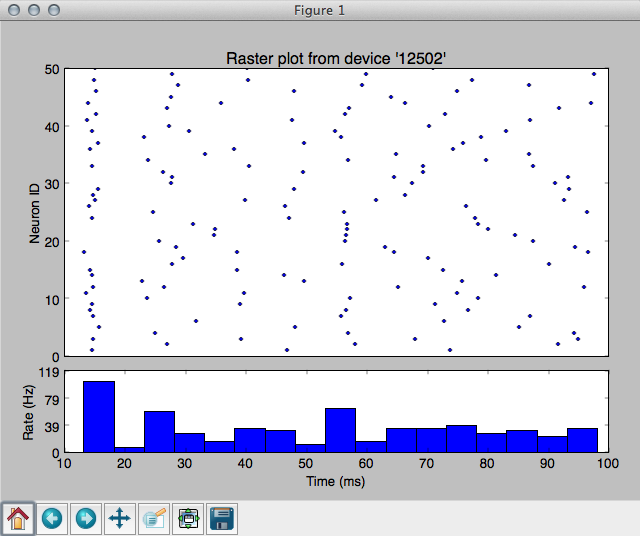
\includegraphics[width=0.9\columnwidth]{../pics/nest_raster.png}
\end{center}

%_________________________________Brian_______________________________________
\ndproject{Brian}{http://www.briansimulator.org/}{brian_logo.png}{.3}{0em}{-2.5em}

Brian is a simulator for spiking neural networks. The focus is on making the writing of simulation code as quick and easy as possible for the user, and on flexibility: new and non-standard models are no more difficult to define than standard ones. This allows scientists to spend more time on the details of their models, and less on their implementation. Neuron models are defined by writing differential equations in standard mathematical notation, facilitating scientific communication. Brian is written in the Python programming language, and uses vector-based computation as well as C code generation to allow for efficient simulations. It also comes with libraries for auditory modelling and fitting neural models to data. Brian is particularly useful for neuroscientific modelling at the systems level, and for teaching computational neuroscience.

\begin{center}
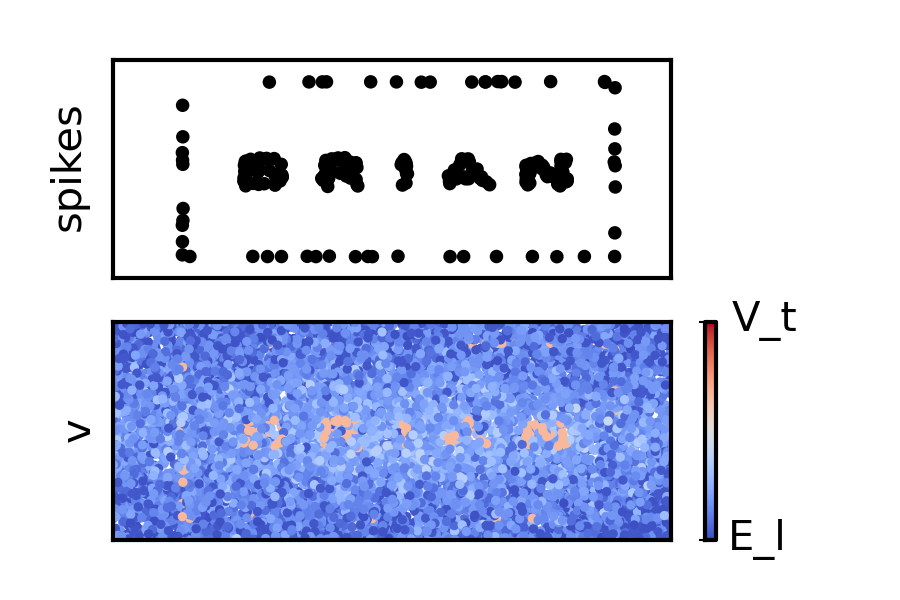
\includegraphics[width=\columnwidth]{../pics/brian_raster.png}
\end{center}
%________________________LFPy_______________________________________________

\ndproject{LFPy}{http://compneuro.umb.no/LFPy}{lfpy_logo.pdf}{.3}{-0.25em}{-3em}

LFPy is a Python module for simulation of extracellular electrical
potentials evoked by activity of multi-compartment model neurons.
LFPy runs on top of the NEURON-simulator, using the included Python interface
(\url{http://www.neuron.yale.edu}).

LFPy provides:
\begin{itemize}[nolistsep, topsep=0em, leftmargin=1pc]
\item A forward modeling scheme for calculating extracellular potentials from compartmental membrane currents in an infinite homogeneous linear extracellular medium.
\item Simple to use Python-classes for setting up cells, synapses and recording electrodes.
\item Easy to use scripting capabilities thanks to NEURON and the Python programming environment.
\item Functionality to employ or specify biophysically detailed model neurons, add a stimulus, and perform a simultaneous simulation of the model cell responses and extracellular potentials.
\item Support for common formats for reconstructed neuronal morphologies, allowing use of publicly available 3D-reconstructions (e.g., \url{http://www.neuromorpho.org}). 
\end{itemize}


\ndsection{Meta-simulators}%

%_________________________________PyNN_______________________________________
\ndproject{PyNN}{http://neuralensemble.org/PyNN/}{neurosharelogo_square.png}{.2}{-0.25em}{0em}

STUFF

\begin{itemize}[nolistsep,topsep=0em,leftmargin=1pc]
\item ITEM 1
\item ITEM 2
\end{itemize}

%_________________________________neuroConstruct_______________________________________
\ndproject{neuroConstruct}{http://www.neuroconstruct.org/}{neurosharelogo_square.png}{.2}{-0.25em}{0em}

STUFF - written in Java but has a Jython interface

\begin{itemize}[nolistsep,topsep=0em,leftmargin=1pc]
\item ITEM 1
\item ITEM 2
\end{itemize}

%___________________________________________________________________________

\ndsection{Analysis tools}%

%_________________________________neo_______________________________________
\ndproject{Neo}{http://packages.python.org/neo}{neo_logo.pdf}{.4}{-0.25em}{-5em}

Neo provides a common model for representing
electrophysiology data in Python. It provides I/O for reading a wide
range of neurophysiology file formats (Spike2,
NeuroExplorer, AlphaOmega, Axon, Blackrock, Plexon, Tdt) and for
writing to a subset of these formats plus non-proprietary formats
including HDF5.

% The goal of Neo is to improve interoperability between Python tools for analyzing, visualizing
% and generating electrophysiology data (such as OpenElectrophy, NeuroTools, G-node,
% Helmholtz, PyNN) by providing a common, shared object model. In order to be as
% lightweight a dependency as possible, Neo is deliberately limited to represention of data,
% with no functions for data analysis or visualization.

Neo implements a hierarchical data model well-adapted to intracellular
and extracellular electrophysiology and EEG data with support for
multi-electrodes (e.g., tetrodes).  Neo's data objects build on
the \href{http://pypi.python.org/pypi/quantities}{quantities} package,
which in turn builds on \href{http://www.numpy.org}{NumPy} by adding
support for physical dimensions. Thus Neo objects behave like
normal NumPy arrays but with additional metadata, checks for
dimensional consistency and automatic unit conversion.

A project with similar aims but for neuroimaging file formats is
\href{http://www.nipy.org/nibabel}{NiBabel}.

%_________________________________NeuroTools_______________________________________
\ndproject{NeuroTools}{http://neuralensemble.org/}{neurosharelogo_square.png}{.2}{-0.25em}{0em}

STUFF

\begin{itemize}[nolistsep,topsep=0em,leftmargin=1pc]
\item ITEM 1
\item ITEM 2
\end{itemize}

\ndsection{Model description languages}%

%_________________________________libNeuroML____________________________________
\ndproject{libNeuroML}{http://www.neuroml.org}{neurosharelogo_square.png}{.2}{-0.25em}{0em}

STUFF ABOUT Python libNeuroML

\begin{itemize}[nolistsep,topsep=0em,leftmargin=1pc]
\item ITEM 1
\item ITEM 2
\end{itemize}

%_________________________________libNineML____________________________________
\ndproject{libNineML}{http://nineml.incf.org}{neurosharelogo_square.png}{.2}{-0.25em}{0em}

STUFF ABOUT Python lib9ML

\begin{itemize}[nolistsep,topsep=0em,leftmargin=1pc]
\item ITEM 1
\item ITEM 2
\end{itemize}

\end{multicols}
\end{document}

%%% Local Variables:
%%% mode: latex
%%% TeX-master: t
%%% TeX-PDF-mode: t
%%% whizzy-viewers: (("-pdf" "okular") ("-dvi" "xdvi") ("-ps" "gv"))
%%% End:
